\section{Regulator}
\label{sec:kontrollerdeign}
%%%Det gør vi jo ikke, men udkommenteret fordi det var Mikkels første Tikz
% Det er valgt at designe regulatoren efter processen illustreret i figur \ref{fig:designproces}.
% \begin{figure}[!th]
% \centering
% \include*{./graphics/designproces}
% \caption[Designprocessen]{Designprocessen, \citep[Side. 260]{reg_modern_control_systems}.}
% \label{fig:designproces}
% \end{figure}

Formålet med reguleringen er som beskrevet i afsnit \ref{sec:problemformulering},
at kontrollere PTS's position.
I afsnit \ref{sec:kravspecifikation} opstilles kravene til systemets respons.
Disse er opsummeret nedenfor.
\begin{itemize}
\itemsep1pt
\item \(t_{s} \leq 0,557 \text{ [s]}\) (Settling Time)
\item \(TE \leq 1,02\degree\) (Trackingfejl efter \(t_s\))
\end{itemize}

Systemets konfiguration består af en koordinattransformation,
en regulering, en aktuering og en positionsmåling, som illustreret
i figur \ref{fig:digitalkontroller1}.
\begin{figure}[!th]
\centering
% \begin{tikzpicture}[auto, node distance=2.6cm,>=latex']
\begin{tikzpicture}[scale=0.8, every node/.style={scale=0.8}, node distance=2.6cm, =>latex']
\include*{./graphics/digitalkontroller1}
\end{tikzpicture}
\caption[Systemkonfiguration]{Systemkonfiguration (blokdiagram).
	Området markeret med rød stiplet linje udgør den digitale regulator.
	De grønne ovaler angiver "clocksignaler", som leverer pulser til de digitale dele af systemet.}
\label{fig:digitalkontroller1}
\end{figure}

Som beskrevet i afsnit \ref{sec:problemformulering},
så er input-samplingen fastlagt til at foregå med en frekvens på 120 [Hz].
Men som illustreret på figur \ref{fig:digitalkontroller1}, så skal reguleringssløjfen
"køres" (sample) med en frekvens \(f_s=\frac{1}{T_s}\), der ikke nødvendigvis er 120 [Hz].
Dvs. D/D- D/A- og A/D-konverteringerne (på nær input-samplingen) skal foregå med frekvensen \(f_s\).

Der er overordnet to strategier til valg af samplingfrekvensen \(f_s\) hvormed
reguleringssløjfen skal køre:
1) Hvis man designer en kontinuert regulator til det kontinuerte domæne, så
skal diskretiseringen af controlleren være så tæt på den kontinuerte regulator som muligt.
Det vil sige, samplingfrekvensen skal vælges så høj som mulig.
2) Hvis man derimod designer en diskret regulator til det diskrete domæne,
så er diskretiseringen allerede foretaget inden designet af regulatoren.
Dvs. man finder en diskretiseret model af det fysiske system inden designet af regulatoren.
Kravet til diskretiseringen af åbensløjfeoverføringsfunktionerne er, at den diskrete repræsentation
skal være tilfredsstillende tæt på de kontinuerte overføringsfunktioner.
Hvis den diskrete overføringsfunktion eksempelvis afviger 20 \% fra den kontinuerte, ville man
sandsynligvis overveje at benytte en højere samplingfrekvens til diskretiseringen.
Sammenligningen af den diskrete overførselsfunktion og den kontinuerte overføringsfunktion
kan være både i tidsdomænet (fx steprespons) og i frekvensdomænet (frekvensrespons, fx. Bode-plots).
Når man har den diskretiserede model af systemet, kan man i det diskrete domæne (z-domænet)
udvikle en regulator - denne er altså diskret fra starten.

Da reguleringen foregår i en task på mikrocontrolleren, vælges det
at udvikle en diskret regulator efter en diskretiseret model af systemet.
Således kan perioden hvormed regulerings-task'en skal køre, fastlægges ud fra
samplingperioden \(T_s\) af diskretiseringen. Hvis man havde valgt at designe en kontinuert regulator
ville perioden skulle vælges så lav som muligt, og dette ville stille højere krav
til mikrocontrolleren.

\subsection{Diskretisering af åbensløjfeoverføringsfunktionerne}
Som beskrevet ovenfor ønskes det at finde en diskretiseret overføringsfunktion
for det fysiske system. Den kontinuerte del af systemet, som ønskes diskretiseret,
er markeret på figur \ref{fig:digitalkontroller2}.
\begin{figure}[!th]
\centering
% \begin{tikzpicture}[auto, node distance=2.6cm,>=latex']
\begin{tikzpicture}[scale=0.8, every node/.style={scale=0.8}, node distance=2.6cm, =>latex']
\include*{./graphics/digitalkontroller2}
\end{tikzpicture}
\caption[Diskretisering af åbensløjfeoverføringsfunktion]{Diskretisering af åbensløjfdeoverføringsfunktion.
	Den kontinuerte del af systemet (markeret med rød stiplet linje) ønskes diskretiseret.
	De grønne ovaler angiver "clocksignaler", som leverer pulser til de digitale dele af systemet.}
\label{fig:digitalkontroller2}
\end{figure}

Den diskretiserede åbensløjfeoverføringsfunktion fra duty cycle til output vinkel
benævnes \(G_{zoh}\left(z\right)\). Dette er fordi D/A-konverteringen modelleres som et Zero Order Hold kredsløb,
der fastholder en analog spænding proportional med duty cyclen. Dette stemmer overens med den simplificerede
model for PWM-signalet beskrevet i afsnit \ref{subsec:matFPGA}.
Den diskrete overføringsfunktion \(G_{zoh}\left(z\right)\) plads i blokdiagrammet for systemet
er indtegnet i figur \ref{fig:digitalkontroller3}.
\begin{figure}[!th]
\centering
% \begin{tikzpicture}[auto, node distance=2.6cm,>=latex']
\begin{tikzpicture}[scale=0.9, every node/.style={scale=0.9}, node distance=2.6cm, =>latex']
\include*{./graphics/digitalkontroller3}
\end{tikzpicture}
\caption[Diskretiseret åbensløjfeoverføringsfunktion]
		{Diskretiseret åbensløjfeoverføringsfunktion.
		\(G_{zoh}\left(z\right)\) erstatter den kontinuerte del af systemet.}
\label{fig:digitalkontroller3}
\end{figure}

Kravet til \(G_{zoh,pan}\left(z\right)\) og \(G_{zoh,tilt}\left(z\right)\) er, at de
med god tilnærmelse opfører sig som \(G_{pan}\left(s\right)\) og \(G_{tilt}\left(s\right)\),
og dette krav kan skrives som et mindstekrav til samplingfrekvensen \(f_s\).

\subsubsection{Valg af samplingfrekvens}\label{subsec:choosefs}
Reguleringssløjfen skal køre periodisk på mikroprocessoren
med samplingfrekvensen \(f_s\). \\
\(f_s\) skal vælges
ud fra systemets dynamik,
%(til diskretiseringen), 
fra inputparablens egenskaber samt 
mikrocontrollerens begrænsninger. 
Inputparablen er samplet ved 120 [Hz], 
\(f_s\) skal derfor være større end 120 [Hz] for at bevare inputsignalets integritet \citep[Side. XXX]{dsp}. 
\todo[inline, color=red!20]{find sidetal i dsp bog}
Diskretiseringen af åbensløjfeoverføringsfunktionerne stiller også krav til samplingfrekvensen.
%Diskretiseringen skal altså sammenlignes med den kontinuerte overføringsfunktion.
Det vælges at sammenligne diskretiseringen af det fysiske system med det kontinuerte system i tidsdomænet.
% Sløjfen lukkes med en forstærkning på 1, og step-responsens karakteristik sammenlignes
% for den diskretiserede overføringsfunktion \(\frac{G_{zoh,tilt}}{1+G_{zoh,tilt}}\)
% og for den kontinuerte overføringsfunktion \(\frac{G_{tilt}}{1+G_{tilt}}\) (en tilsvarende sammenligning foretages for pan).
Sløjfen lukkes med en forstærkning på 1, 
og step-responsens karakteristik for den diskrete og kontinuere overføringsfunktion sammenlignes. 
% Diskretiseringen opfører sig med bedste tilnærmelse som det kontinuerte system
% når Rise Time, Settling Time og Overshoot efter diskretiseringen
% ændrer sig så lidt som muligt i forhold til responsen af det kontinuerte system.
Diskretiseringen vurderes at være tæt nok på den kontinuere model, hvis følgende krav opfyldes:
Det vurderes, at Rise Time og Settling Time maks. må ændre sig med 5\% i forhold
til den kontinuerte respons, mens at Overshoot maks. må ændre sig med 25\% i forhold til
den kontinuerte respons.

\begin{figure}
 \centering
\begin{tabular}{lr}
 Overshoot & 25\%\\
 Rise Time & 5\%\\
 Settling Time & 5\%\\
\end{tabular}
\caption{fejl}
\end{figure}
\todo[inline, color=red!20]{skal rettes til}

Hvis diskretiseringen kræver at reguleringssløjfen kører ved en frekvens \(f_s\),
der er højere end A/D-konverteringens 120 [Hz], skal det A/D-konverterede
signal "upsamples" til \(f_s\).
Upsamplingen er simplest at implementere
hvis \(f_s\) er et heltalsmultiplum af (120 [Hz]) \citep[Side. 562]{dsp}.
Det vælges derfor at sample ved et heltalsmultiplum \(f_s\) af 120 [Hz].

På figur \ref{fig:diskretTiltStep} er stepresponsen for lukketsløjfesystemet (med forstærkning 1)
med \(G_{tilt}\) indtegnet sammen med den tilsvarende steprespons for tre forskellige diskretiseringer
af \(G_{tilt}\). Som det ses af grafen, er det diskretiserede systems respons tættest
på det kontinuerte systems respons når samplingfrekvensen er højest.
\begin{figure}[!th]
\centering
	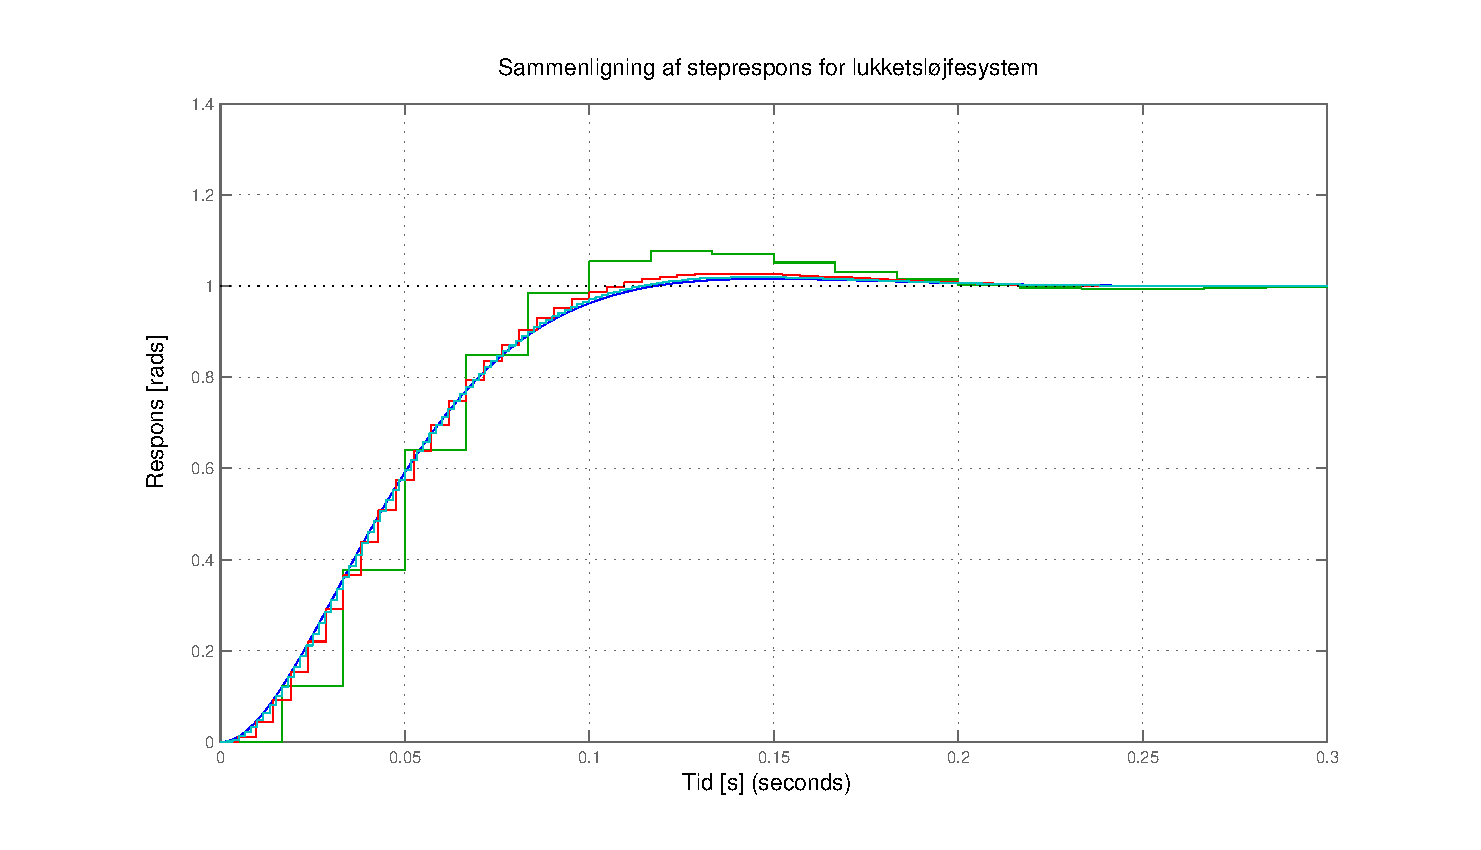
\includegraphics[width=0.8\textwidth]{./graphics/diskretTiltStep.eps}
	\captionsetup{width=0.7\textwidth}
\caption[Sammenligning af steprespons performance]
{Sammenligning af steprespons for kontinuert system med diskretiseret system.
Den mørkeblå kurve er det kontinuerte systems respons,
og de andre kurver er det diskretiserede systems respons ved en samplingfrekvens på
120 [Hz] (grøn), 240 [Hz] (rød) og 600 [Hz] (lyseblå).}
\label{fig:diskretTiltStep}
\end{figure}
På figur \ref{fig:diskretStepFreq} er samme steprespons' performance afbildet
for pan og for tilt som funktion af samplingfrekvensen \(f_s\).
De sammenlignede størrelser er Rise Time, Settling Time og Overshoot.
Graferne viser ændringen af de tre størrelser i procent i forhold til det kontinuerte systems respons.
\begin{figure}[!th]
\centering
	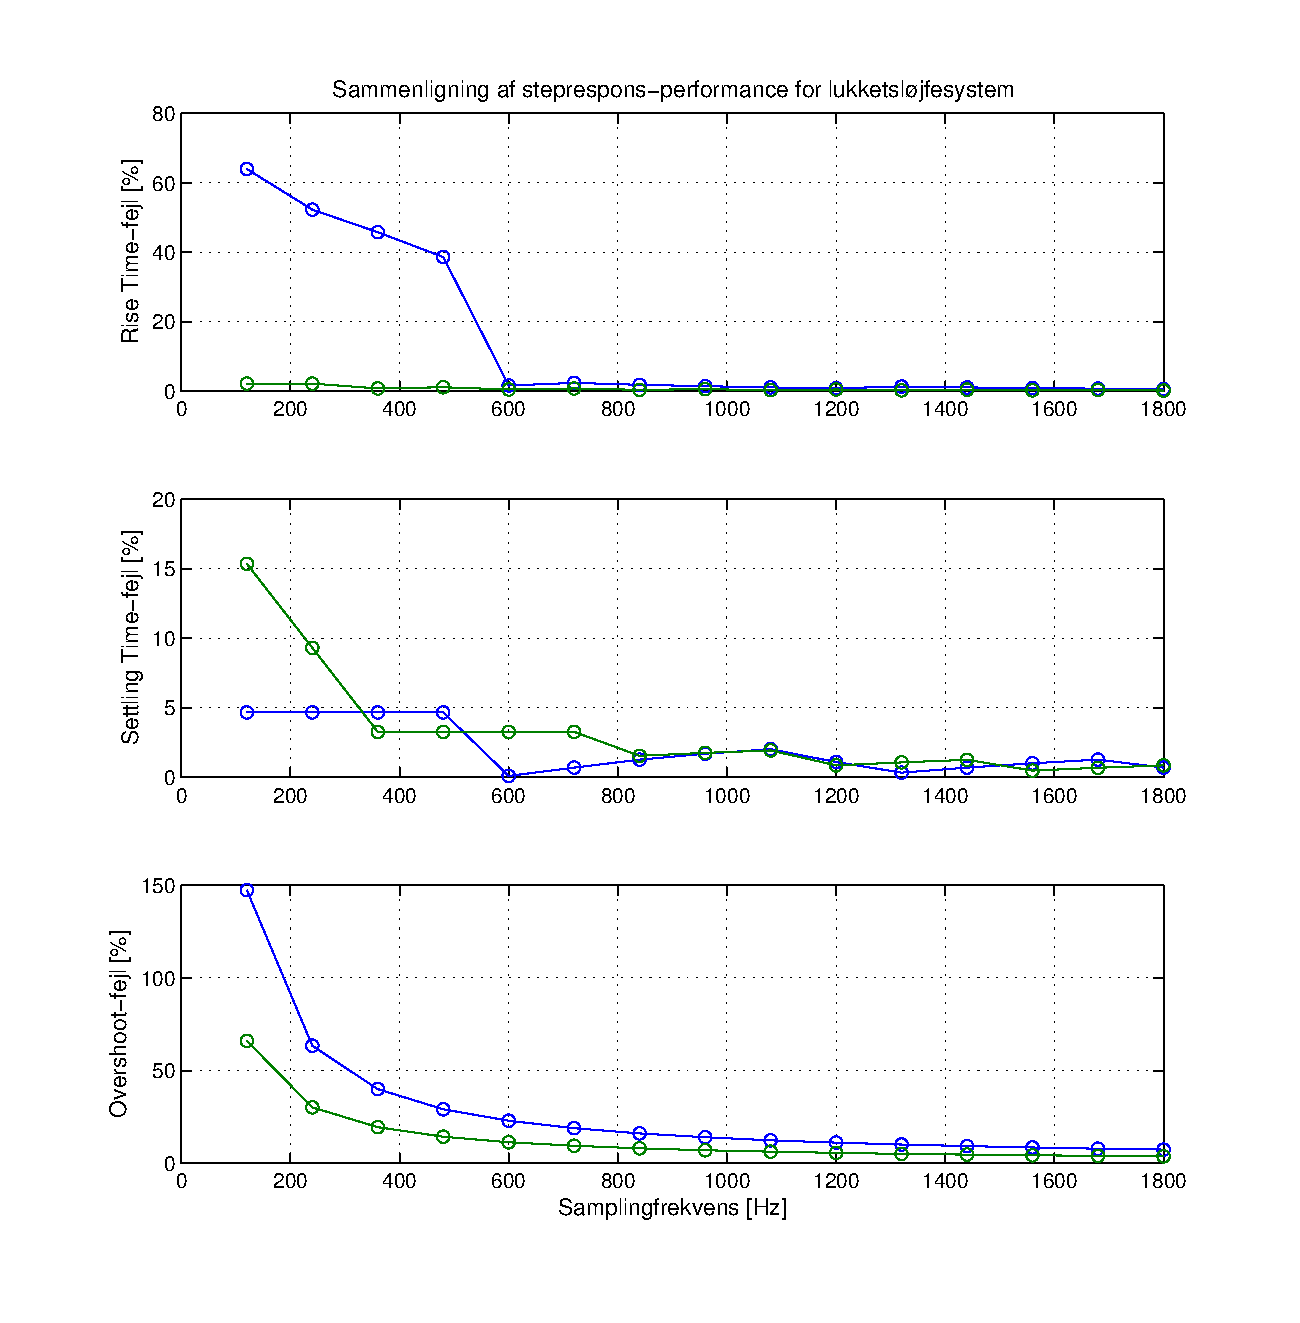
\includegraphics[width=1\textwidth]{./graphics/diskretStepFreq.eps}
%\caption[Sammenligning af steprespons-performance for kontinuert system med diskretiseret system (\(G_{zoh}\))]
%{Sammenligning af steprespons-performance for kontinuert system med diskretiseret system.
%Den blå kurve angiver fejlen i forhold til lukketsløjferesponsen af \(G_{tilt}\),
%mens den grønne kurve angiver fejlen i forhold til lukketsløjferesponsen af \(G_{pan}\).
%}

\caption[Sammenligning af steprespons-performance for kontinuert system med diskretiseret system $G_{zoh}$]
{Sammenligning af steprespons-performance for kontinuert system med diskretiseret system.
Den blå kurve angiver fejlen i forhold til lukketsløjferesponsen af $G_{tilt}$,
mens den grønne kurve angiver fejlen i forhold til lukketsløjferesponsen af $G_{pan}$.
}
\label{fig:diskretStepFreq}
\end{figure}

Som forventet kan et generelt mønster ses på graferne i figur \ref{fig:diskretTiltStep} og figur \ref{fig:diskretStepFreq}:
Jo højere samplingfrekvens, jo tættere kommer diskretiseringens respons på det kontinuerte systems respons.
En yderligere inspicering viser, at en særligt god performance opnås ved en samplingfrekvens på 600 [Hz],
hvor kravene til diskretiseringens performance opfyldes.

Figur \ref{fig:diskretTiltStep} og figur \ref{fig:diskretStepFreq}
giver et grundlag for valg af reguleringssløjfens samplingfrekvens ud fra det fysiske systems dynamik.
Hvis mikrocontrollerens begrænsninger tages med i betragtning vil man vælge den lavest acceptable
samplingfrekvens.

Som udgangspunkt vælges derfor en samplingfrekvens på \(f_s=600 \text{ [Hz]}\),
så diskretiseringen med god tilnærmelse har samme performance som det kontinuerte system.

\subsubsection{Analyse af den diskretiserede overføringsfunktion}
I ligningerne \ref{eq:transpantilt1} findes de diskretiserede overføringsfunktioner.
\begin{align}
\label{eq:transpantilt1}
\begin{split}
	G_{zoh,pan}\left(z\right)&\approx\frac{7,94\cdot{}10^{-4}\cdot{}z^2
							+1,56\cdot{}10^{-3}\cdot{}z
							+1,18\cdot{}10^{-4}}
							{z^3 - 1,95\cdot{}z^2+9,67\cdot{}10^{-1}\cdot{z}-1,76\cdot{}10^{-2}}
	\\
	\\
	G_{zoh,tilt}\left(z\right)&\approx\frac{1,04\cdot{}10^{-3}\cdot{}z^2
							+2,03\cdot{}10^{-3}\cdot{}z
							+1,54\cdot{}10^{-4}}
							{z^3 - 1,93\cdot{}z^2+9,47\cdot{}10^{-1}\cdot{z}-1,76\cdot{}10^{-2}}
\end{split}
\end{align}
 
Den i afsnit \ref{subsec:choosefs} udførte sammenligning af det diskretiserede systems performance
med det kontinuerte systems performance viser,
at Rise Time stiger med 3,3 \% for pan og 0,10 \% for tilt,
Settling Time stiger med 0,48 \% for pan og 1,6 \% for tilt,
samt at Overshoot stiger med 11 \% for pan og 23 \% for tilt
ved lukketsløjfesystemet med en forstærkning på 1.
Diskretiseringen sammenlignes i frekvensdomænet med det kontinuerte system
i figur \ref{fig:diskretBode}, der viser Bode-plot for \(G_{pan}\) og \(G_{tilt}\) samt
deres diskretiseringer (ved 600 [Hz]) \(G_{zoh,pan}\) og \(G_{zoh,tilt}\).
\todo[inline, color=red!20]{lav om til tabel form}
\begin{figure}[!th]
\centering
	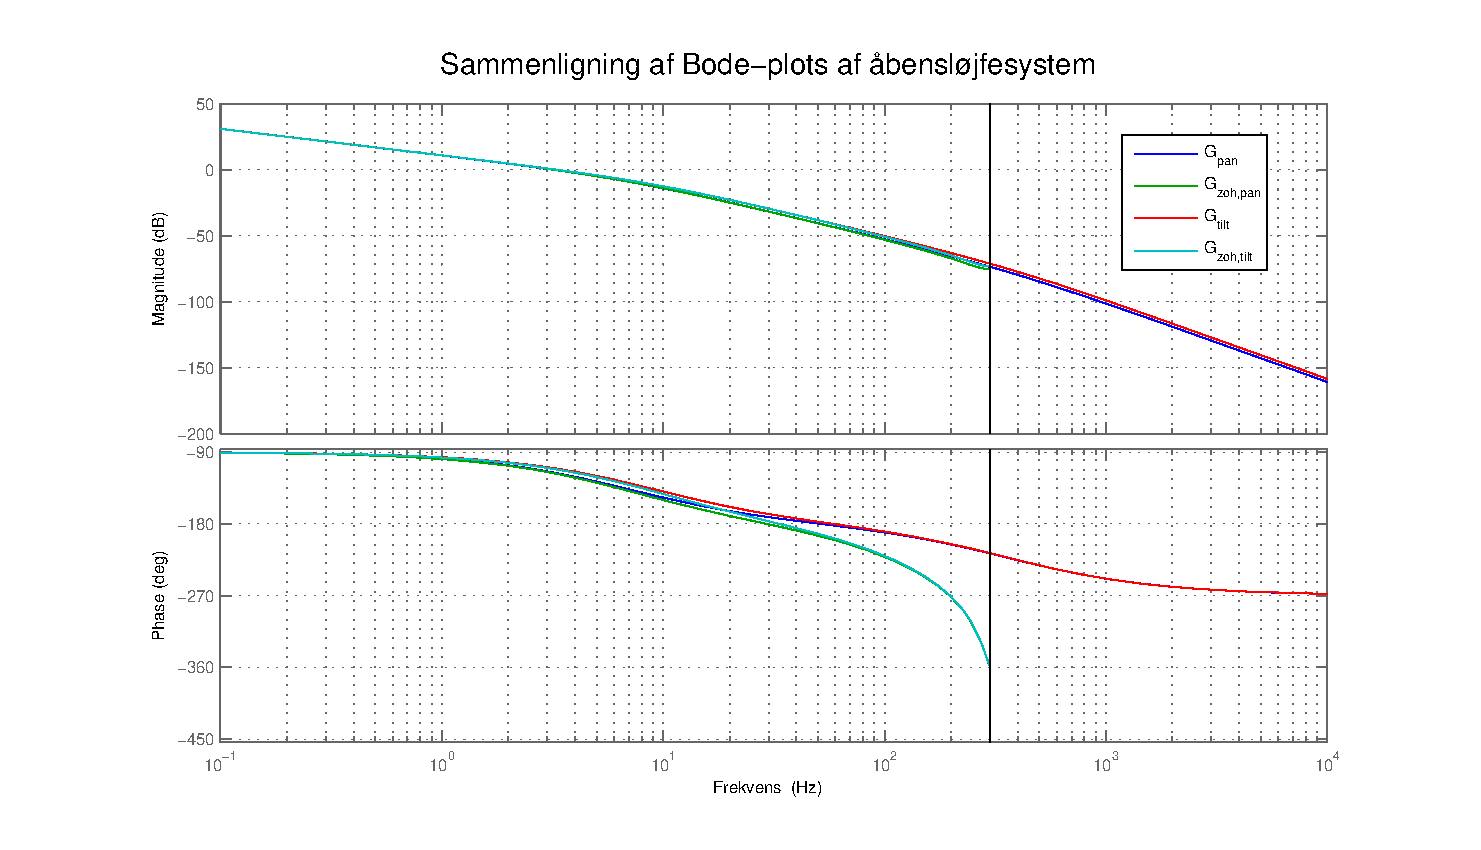
\includegraphics[width=0.8\textwidth]{./graphics/diskretBode.eps}
	\captionsetup{width=0.7\textwidth}
\caption[Sammenligning af Bode-plots]
{Sammenligning af Bode-plots af kontinuert system med diskretiseret system.
Den blå og den røde kurve angiver hhv. \(G_{pan}\) og \(G_{tilt}\) mens
den grønne og den turkise kurve angiver hhv. \(G_{zoh,pan}\) og \(G_{zoh,tilt}\).
}
\label{fig:diskretBode}
\end{figure}
Bemærk at figur \ref{fig:diskretBode} er en sammenligning af \textit{åben}sløjfeoverføringsfunktionernes
frekvensrespons.

Som det ses på grafen, følger det diskretiserede systems respons meget nøje det kontinuerte systems respons.
Fejlen på størrelsen af responsen er meget lille i hele spektret,
mens fejlen på fasen er lille ved lave frekvenser og stiger ved høje frekvenser.

\subsection{Upsampling}
\label{subsec:upsampling}
Da reguleringssløjfen, som beskrevet i afsnit \ref{subsec:choosefs}, køres med en frekvens på 600 [Hz],
som er 5 gange højere end input-samplingfrekvensen, skal der foretages en upsampling.
%Upsamplingen foretages med Zero Order Hold, hvorved ét sample ved 120 Hz indsættes 
%som 5 samples ved 600 Hz.
Upsamplingen indsætter mellem hvert input-sample 4 samples med værdien 0, så hvert input-sample
kun samples én gang. Dette gør, at input-signalets frekvensspektrum bevares.
Da input-signalet er samplet ved 120 [Hz] vil det oprindelige spektrum, centreret omkring 0 [Hz],
spejles ved heltalsmultipla af 120 [Hz]. Disse spejlbilleder af det oprindelige spektrum vil være
indeholdt i det upsamplede signal, hvis det ikke lavpasfiltreres. 
Det vælges at filtrere det upsamplede signal med et Zero Order Hold,
således at de indsatte samples med værdien 0 erstattes med værdien af sidste sample
med en værdi forskellig fra 0. Dette fjerner ikke de førnævnte spejlbilleder, men forøger
til gengæld heller ikke forsinkelsen af input-signalet.

\subsection{Valg af regulatortype}
\label{ss:ValgReg}
Pga. de simplificerende antagelser som er indeholdt i den matematiske model for systemet,
vil en åbensløjferegulering være et dårligt valg: den vil være følsom overfor afvigelser fra den
matematiske model. Desuden er der fra projektoplægget krav om en lukketsløjferegulering.
Den simpleste regulering ville være en konstant forstærkning af fejlsignalet.
De største krav stilles til systemets responstid og ikke så meget til udsvinget af responsen,
og som udgangspunkt vælges derfor en PI-regulator.
Hvis det er nødvendigt at nedjustere udsvinget kan det være nødvendigt at anvende en PID-regulator,
og derfor implementeres algoritmen til en PID-regulator på mikrocontrolleren.
Hvis kun en PI-regulator er nødvendigt, kan man altså blot nulstille D-leddet.

\subsubsection{Dødzone}
Da motorerne ikke kan rotere ved lave spændinger indeholder systemet dødzoner.
Det er valgt at implementere "bias", der tager højde for dødzonerne.
Bias er implementeret symmetrisk med en nedre duty cycle grænse på 0,98\% for pan og tilt.
Deres respektive øvre grænser er hhv. 11,72\% og 14,65\%.
Disse værdier er fundet eksperimentelt.
Hvis regulatoren returnerer en duty cycle mellem den nedre og øvre grænse, sættes duty cycle til dens øvre grænse.
Dette medfører at motoreren kan justere sig ind, selvom fejlen er marginal.

\subsubsection{Integratormætning}
Mætningen på PWM-duty cyclen gør, at systemet ikke er lineær i dette område. Med integratormætning 
tages der delvist højde for denne ulinearitet. Uden integratormætning kan det numeriske integrale blive enormt når 
PWM-mætningen nås. Dette vil føre til stort overshoot og derved dårlig 
performance. 
En for lille integratormætning vil mindske effekten af integratorleddet i PID, 
hvilket i værste tilfælde vil sætte integratorleddet ud af funktion.
En for høj værdi vil føre til at tilføjelse af integratormætningen ikke vil ændre 
performance.

%Et passende valg af integratormætning vurderes til at være når ligning \ref{eq:integratorsaturation} 
%overholdes.

%\begin{equation}
%	K_I \cdot Integrator_{Max} \approx PWM_{Max}
%\label{eq:integratorsaturation}
%\end{equation}
%\todo[inline,author=Mikkel,color=Pink]{Jeg mangler kilde for ovenstående, men kan ikke finde noget. Det er bare mit bedste bud.}

